\documentclass[english]{finalproject}

\captionsetup{labelfont={bf}}

\date{\today}

\usepackage{xkeyval}

\makeatletter

\define@boolkey{load}{all}     [true]{}
\define@boolkey{load}{base}    [true]{}

\define@boolkey{load}{korean}  [true]{}
\define@boolkey{load}{listings}[true]{}
\define@boolkey{load}{math}    [true]{}
\define@boolkey{load}{std}     [true]{}
\define@boolkey{load}{task}    [true]{}
\define@boolkey{load}{tikz}    [true]{}
\define@boolkey{load}{util}    [true]{}

\newcommand{\load}[1]{%
  % set keys
  \presetkeys{load}{base}{}
  \setkeys{load}{#1}

  \ifKV@load@base
    \presetkeys{load}{math,std,task}{}
  \fi

  \ifKV@load@all
    \presetkeys{load}{listings,math,std,task,tikz}{}
  \fi

  \setkeys{load}{#1}

  % load packages
  \ifKV@load@korean
    \usepackage{kotex}
  \fi

  \ifKV@load@listings
    \usepackage{listings}
    \lstset{ basicstyle  = \footnotesize
           , captionpos  = b
           , frame       = lines
           , numbers     = left
           , numberstyle = \tiny
           }
  \fi

  \ifKV@load@math
    \usepackage{amsmath}
    % \usepackage{amssymb} % conflicts with mathdesign loaded in finalproject.cls
    \usepackage{nicefrac}
    \usepackage{siunitx}

    \DeclareMathOperator{\fl}{fl}
    \DeclareMathOperator{\range}{range}
    \DeclareMathOperator{\rank}{rank}
  \fi

  \ifKV@load@std
    \usepackage{booktabs}
    \usepackage{enumitem}
    \usepackage[iso]{isodate}
    \usepackage[all]{nowidow}
    \usepackage[super]{nth}
    \usepackage[caption = false, font = small]{subfig}

    \usepackage{hyperref}
    \hypersetup{ colorlinks = true
               , citecolor  = black
               , linkcolor  = black
               , urlcolor   = black
               }
    \def\UrlBreaks{\do\/\do-}

    \setlength{\parindent}{0mm}
  \fi

  \ifKV@load@task
    \usepackage[most]{tcolorbox}
    \newtcolorbox[auto counter]{task}
      { title           = {Task~\thetcbcounter \par}
      , before          = {\bigskip}
      , after           = {\medskip}
      , fonttitle       = {\scshape}
      , colback         = {black!5!white}
      , coltext         = {black}
      , coltitle        = {black}
      , borderline west = {3pt}{0pt}{black}
      , frame hidden
      , boxrule         = 0mm
      , boxsep          = 0mm
      , enhanced jigsaw
      , attach title to upper
      }
  \fi

  \ifKV@load@tikz
    \usepackage{pgfplots}
    \pgfplotsset{compat=1.17}
    \usepackage{tikz}
    \usetikzlibrary{calligraphy,decorations.pathreplacing,patterns}
    \usepgfplotslibrary{colorbrewer}
  \fi

  \ifKV@load@util
    \usepackage[ backend=biber
               , bibstyle=ieee
               , citestyle=numeric-comp
               , sortcites=true
               , maxbibnames=30
               , bibencoding=utf8
               , alldates=comp
               ]{biblatex}
    \usepackage{multicol}
    \usepackage{todonotes}
  \fi

  \ifKV@load@std
    % cleveref needs to be loaded last
    \usepackage[capitalise, noabbrev]{cleveref}
  \fi
}

\makeatother

\newcommand{\der}[3][]{\frac{\partial #1 #2}{\partial #3 #1}}
\newcommand{\diff}{\mathop{}\!\mathrm{d}}
\newcommand{\mat}[1]{\begin{pmatrix}#1\end{pmatrix}}
\renewcommand{\qed}{\hfill \ensuremath{\square}}
\newcommand{\shall}{\overset{!}{=}}
\newcommand{\vct}[1]{\boldsymbol{#1}}

\load{util, tikz}
\definecolor{ofs}{HTML}{d291c5}
\definecolor{tfi}{HTML}{7fc6dc}
\definecolor{ifo}{HTML}{7ccd9e}
\definecolor{ifi}{HTML}{255d67}
\definecolor{ofo}{HTML}{663349}
\definecolor{dir}{HTML}{d86d26}
\definecolor{highlight}{HTML}{d73d2c}
\definecolor{upward}{named}{gray}
\definecolor{downward}{named}{yellow}
\newcommand{\dirColor}{\textit{Orchid Crayola} }
\newcommand{\ofsColor}{\textit{Sky Blue} }
\newcommand{\ofoColor}{\textit{Eton Blue} }
\newcommand{\ifoColor}{\textit{Midnight Green} }
\newcommand{\ifiColor}{\textit{Old Mauve} }
\newcommand{\tfiColor}{\textit{Chocolate Web} }
\newcommand{\highlightColor}{\textit{CG Red} }
\newcommand{\upwardColor}{\textit{gray} }
\newcommand{\downwardColor}{\textit{yellow} }


% Title (and subtitle) of the project
\title{Fast Multipole Methods}
%\subtitle{(optional subtitle)}

% Group members for the final project (comment out the unnecessary entries)
\begin{groupmembers}
\studentA{Daniel }{}{Bauer  }
\studentB{Glejdis}{}{Shkëmbi}
\studentC{Michael}{}{Zikeli }
\end{groupmembers}

\newacronym{fmm}{FMM}{Fast Multipole Method}

\abstract {
  The Fast Multipole Method is a numerical technique developed to decrease the time complexity of calculating long-ranged forces in N-body simulation problems.
  In contrast to typical N-body problem solvers, which require $\mathcal{O}(N ^ 2)$ operations, the Fast Multipole Method runs in linear time, without severely compromising accuracy.
  There are several other applications where the Fast Multipole Method reduces the complexity to $\mathcal{O}(N)$, such as matrix-vector multiplication, LU-factorization or acceleration of the iterative solver in the method of moments.
  Within this report, we introduce the Fast Multipole Method for the gravitational N-body problem from a theoretical point of view and implement a 2D spiral galaxy simulation using the Fast Multipole Method with adaptive trees.
  The initial build of the tree requires a time of $\mathcal{O}(N \log N)$ while for the main Fast Multipole Method we achieve linear complexity $\mathcal{O}(N)$.
}

\begin{document}
  \maketitle

  \section{Introduction} \label{introduction}

The \gls{fmm} was first introduced by Greengard and Rokhlin in 1987 for the N-body simulation problem with pairwise interactions, such as elasticity, gravitation, electrostatics, or wave propagation \cite{Greengard1987AFA, Martinsson2015}.
N-body problems typically have a complexity of $\mathcal{O}(N^2)$ \cite{SicchaSeminar}.
The \gls{fmm} solves this problem by introducing an approximation of the driving force term, achieving linear complexity \cite{Martinsson2015}.
Moreover, the \gls{fmm} uses quad-trees or oct-trees to hierarchically split the computing domain and thus is frequently referred to as a ``tree code'' algorithm.
The tree structure makes this algorithm well-suited for multi-core and parallel computing systems \cite{Martinsson2015}.
This report first sheds some light on the inner workings of the FMM by providing in depth details on the steps of the algorithm and analyzing its time complexity.
Afterwards, the operators used by the algorithm are introduced and a rough analysis of the approximation error is given.
Lastly, details of the implementation of the rotating galaxy simulation are shown, as well as the obtained results.
After reading the report, the reader should comprehend the algorithm’s underlying concepts and understand how the linear time complexity is achieved.

In this paper, we consider $N$ particles $p_i$ placed at positions $\vct x_i \in \Omega \subset \mathbb{R}^2$, where $\Omega$ is a rectangular domain.
For the ease of notation, we think of $\vct x_i$ as a point in the complex plane, where $\Re(\vct x)$ is the real part of $\vct x$.
Each of these particles induces a long-range potential $\Psi_i(\vct x) = m_i \log(\vct x - \vct x_i)$, where $m_i$ is the mass of the source particle $p_i$.
The aim is to obtain the net force $\vct f_j$ acting on the target particle $p_j$, which is the sum of all pairwise interactions \cite{short-course}:
\begin{equation}
  \vct f_j = \sum_{i=1, i\neq j}^N \vct F_{ij}(\vct x_i - \vct x_j, m_i m_j)
      = -\sum_{i=1, i\neq j}^N m_j \nabla \Re(\Psi_i(\vct x_j))
  \label{equ:force}
\end{equation}

  \section{The Algorithm}
\label{algorithm}

\newcommand\scaleFigures{0.8} % this variable defines how the figures for the steps are scaled, relatively to the chosen size.

This section focuses on explaining the \gls{fmm} algorithm by introducing the underlying data structure and giving a step by step introduction of its necessary operations.
The general idea behind the algorithm is to reduce the number of pairwise interactions by introducing approximations representing entire ``clusters'' of interactions.
By doing so, each of the $N$ target particles $p_j$ immediately interacts with only a few close particles, for all other ``distant'' interactions, the approximations are considered.

\subsection{A Tree of Boxes, Neighbors and Interaction Lists}

To achieve linear complexity, the \gls{fmm} utilizes a tree based structure, in our 2D case a quad-tree.
The root node of the tree corresponds to the domain $\Omega$.
From the root, the domain is recursively subdivided in four equal-sized nodes until every node contains less than $s$ particles.
Nodes that do not need further refinement are called the leafs or leaf nodes of the tree \cite{Martinsson2015}.

Given two distinct nodes $\sigma,\tau$, we define the following \cite{Martinsson2015}:
\begin{description}
  \item[The parent] of $\tau$ is the node on the next coarser level that contains $\tau$.
  \item[The children] of $\tau$ compose the set $\mathcal{L}_{\tau}^\text{child}$ of nodes with $\tau$ as their parent.
  \item[The neighbors] of $\tau$ compose the set $\mathcal{L}_{\tau}^\text{nei}$ of nodes on the same level that directly touch $\tau$.
  \item[The interaction list] of $\tau$ is the set $\mathcal{L}_{\tau}^\text{int}$ of all nodes $\sigma$ such that $\sigma$ and $\tau$ are on the same level, and do not touch each other, but their parents touch each other.
  \item[$\sigma$ is well-separated] from $\tau$ if they are on the same level and not neighbors.
\end{description}

\subsection{The Fast Multipole Method}

In the following, we elaborate on the main steps of the algorithm as described by Martinsson in \cite{Martinsson2015}, the mathematical details are given in \cref{operators}.

\begin{enumerate}
  \setcounter{enumi}{-1}

  \item \textbf{Construct the tree and all interaction lists.}
    \\
    Before calculating any forces, we need to build the tree data structure and determine the interaction lists, as described above.
    This has complexity $\mathcal{O}(N\log{N})$, however, it needs to be done only once during the initialization. Hence, for a sufficiently long simulation, this initial effort can be neglected.
    \\
    \cref{fig:tree} shows how the information of all source particles $p_i$ propagates to the target particles $p_j$.
    The differently colored arrows in this figure represent the different steps of the algorithm which are described below.
    \begin{figure}
  \centering
  \null\hfill
  \subfloat{%
    \begin{tikzpicture}[scale=1]
    \pgfmathsetseed{17}

      \coordinate (ydist) at (0,1);
      \coordinate (xdist) at (1,0);

      \coordinate (a) at (0,0);

        \coordinate (b) at ($ (a) - (ydist) - 2*(xdist) $);
        \draw (a) -- (b);

          \coordinate (d) at ($ (b) - (ydist) - (xdist) $);
          \draw (b) -- (d);

            \coordinate (h) at ($ (d) - (ydist) - 0.5*(xdist) $);
            \draw (d) -- (h);
            \coordinate (i) at ($ (d) - (ydist) + 0.5*(xdist) $);
            \draw (d) -- (i);

          \coordinate (e) at ($ (b) - (ydist) + (xdist) $);
          \draw (b) -- (e);

            \coordinate (j) at ($ (e) - (ydist) - 0.5*(xdist) $);
            \draw (e) -- (j);
            \coordinate (k) at ($ (e) - (ydist) + 0.5*(xdist) $);
            \draw (e) -- (k);

        \coordinate (c) at ($ (a) - (ydist) + 2*(xdist) $);
        \draw (a) -- (c);

          \coordinate (f) at ($ (c) - (ydist) - (xdist) $);
          \draw (c) -- (f);

            \coordinate (l) at ($ (f) - (ydist) - 0.5*(xdist) $);
            \draw (f) -- (l);
            \coordinate (m) at ($ (f) - (ydist) + 0.5*(xdist) $);
            \draw (f) -- (m);

          \coordinate (g) at ($ (c) - (ydist) + (xdist) $);
          \draw (c) -- (g);

            \coordinate (n) at ($ (g) - (ydist) - 0.5*(xdist) $);
            \draw (g) -- (n);
            \coordinate (o) at ($ (g) - (ydist) + 0.5*(xdist) $);
            \draw (g) -- (o);

      \foreach \x in { (a), (b), (c)
                     , (d), (e), (f)
                     , (g), (h), (i)
                     , (j), (k), (l)
                     , (m), (n), (o) } {
        \draw[fill] \x circle (2pt);
      }


      \coordinate (step) at (0, 0.8);
      \coordinate (startingPoint) at ($ (h) - (step) $);
      \foreach \i in {0,...,7}{
        \def\radius{0.2}
        \foreach \tmp in {1,...,50} {
          \coordinate (z) at (rnd*2*\radius-\radius, rnd*2*\radius-\radius);
          \draw[fill, black!40] ($ \i*(xdist)+(startingPoint)+(z)$) circle (0.5pt);
        }
      }
      \draw[fill, highlight] ($ 4*(xdist)+(startingPoint)+(z)$) circle (1pt)
        node[right] {\scriptsize\textcolor{black}{$p_j$}};
      \draw[fill, black!40] ($ 3*(xdist)+(startingPoint)+(z)$) circle (1pt)
        node[right] {\scriptsize\textcolor{black}{$p_i$}};

      \draw[fill, tfi] (l) circle (2pt);
      \node[draw=tfi, dashed, inner sep=8pt] at ($ 4*(xdist)+(startingPoint)$){};
      \draw[tfi, thick, ->] ($ (l)-(0,0.1) $)
        -- ($ 4*(xdist)+(startingPoint)+(0,0.4)$)
        node[midway, right] {\scriptsize\textcolor{black}{$\vct{T}_{\tau}^{\mathrm{tfi}}$}};

      \node[draw=dir, dashed, inner sep=8pt] at ($ 3*(xdist)+(startingPoint)$){};
      \draw[dir, thick, ->] ($ 3*(xdist)+(startingPoint)+(0.3,0)$) -- ($ 4*(xdist)+(startingPoint)-(0.3,0)$);
      \node[draw=dir, dashed, inner sep=8pt] at ($ 5*(xdist)+(startingPoint)$){};
      \draw[dir, thick, ->] ($ 5*(xdist)+(startingPoint)-(0.3,0)$) -- ($ 4*(xdist)+(startingPoint)+(0.3,0)$);

      \draw[ifo, thick, ->] ($ (j) + (0.1, +0.05) $)
        .. controls ($ (l) - (xdist) + (0,0.3) $)
        .. ($ (l) + (-0.1, +0.05) $);
      \draw[ifo, thick, ->] ($ (n) + (-0.1, +0.05) $)
        .. controls ($ (l) + (xdist) + (0,0.15) $)
        .. ($ (l) + (0.1, 0) $);
      \draw[ifo, thick, ->] ($ (o) + (-0.1, +0.05) $)
        .. controls ($ (l) + 1.5*(xdist) + (0,0.4) $)
        .. ($ (l) + (0.1, +0.1) $);
      \draw[ifo, thick, ->] ($ (d) + (0.1, +0.05) $)
        .. controls ($ (f) - 2*(xdist) + (0,0.5) $)
        .. ($ (f) + (-0.1, +0.1) $)
        node[midway, above] {\scriptsize\textcolor{black}{$\vct{T}_{\nu,\mu}^{\mathrm{ifo}}$}};

      \draw[ofs, thick, ->] ($ 0*(xdist)+(startingPoint)+(0,0.3)$)
        -- ($ (h) - (0,0.2) $)
        node[midway, right] {\scriptsize\textcolor{black}{$\vct{T}_{\sigma}^{\mathrm{ofs}}$}};

      \draw[ofs, thick, ->] ($ 1*(xdist)+(startingPoint)+(0,0.3)$)
        -- ($ (i) - (0,0.2) $);
      \draw[ofs, thick, ->] ($ 2*(xdist)+(startingPoint)+(0,0.3)$)
        -- ($ (j) - (0,0.2) $);
      \draw[ofs, thick, ->] ($ 6*(xdist)+(startingPoint)+(0,0.3)$)
        -- ($ (n) - (0,0.2) $);
      \draw[ofs, thick, ->] ($ 7*(xdist)+(startingPoint)+(0,0.3)$)
        -- ($ (o) - (0,0.2) $);

      \draw[ofo, thick, ->] ($ (h) + (-0.1,0.1) $)
        -- ($ (d) + (-0.15,-0.05) $);
      \draw[ofo, thick, ->] ($ (i) + (+0.1,0.1) $)
        -- ($ (d) + (+0.15,-0.05) $)
        node[midway, right] {\scriptsize\textcolor{black}{$\vct{T}_{\mu,\sigma}^{\mathrm{ofo}}$}};

      \draw[ifi, thick, ->] ($ (f) - (0.15,0.05) $)
        -- ($ (l) - (0.1,-0.1) $)
        node[midway, left] {\scriptsize\textcolor{black}{$\vct{T}_{\tau,\nu}^{\mathrm{ifi}}$}};

    \end{tikzpicture}
  }
  \hfill\subfloat{%
    \begin{tikzpicture}[scale=0.4]

      \draw[ofs, ->, ultra thick] (0, -0) -- (1, -0) node[right] (l1) {\scriptsize\textcolor{black}{step 1) outgoing from source expansion $\vct{T}_{\sigma}^{\mathrm{ofs}}$}} ;
      \draw[ofo, ->, ultra thick] (0, -1) -- (1, -1) node[right] (l2) {\scriptsize\textcolor{black}{step 2) outgoing from outgoing expansion $\vct{T}_{\mu,\sigma}^{\mathrm{ofo}}$}} ;
      \draw[ifo, ->, ultra thick] (0, -2) -- (1, -2) node[right] (l3) {\scriptsize\textcolor{black}{step 3) incoming from outgoing expansion $\vct{T}_{\nu,\mu}^{\mathrm{ifo}}$}} ;
      \draw[ifi, ->, ultra thick] (0, -3) -- (1, -3) node[right] (l4) {\scriptsize\textcolor{black}{step 4) incoming from incoming expansion $\vct{T}_{\tau,\nu}^{\mathrm{ifi}}$}} ;
      \draw[tfi, ->, ultra thick] (0, -4) -- (1, -4) node[right] (l5) {\scriptsize\textcolor{black}{step 5) target from incoming expansion $\vct{T}_{\tau}^{\mathrm{tfi}}$}} ;
      \draw[dir, ->, ultra thick] (0, -5) -- (1, -5) node[right] (l6) {\scriptsize\textcolor{black}{step 5) immediate computation}} ;
      \draw[fill, highlight] (0.5, -6) circle (3pt) node[right] (l7) at ($ (l6.west) + (0, -1)$){\scriptsize\textcolor{black}{target particles $p_j$}};
      \draw[fill, black!40 ] (0.5, -7) circle (3pt) node[right] (l8) at ($ (l7.west) + (0, -1)$){\scriptsize\textcolor{black}{source particles $p_i$}};

      \node (leftCorner) at ($ (l1.west) + (-1, 0) $) {};
      \node[draw, fit=(leftCorner) (l1) (l2) (l3) (l4) (l5) (l6) (l7) (l8)] {};
    \end{tikzpicture}
  }
  \hfill\null
  \caption{Flow of information through the tree (1D case)}
  \label{fig:tree}
\end{figure}

    \label{it:init}

  \item \textbf{Outgoing from source expansion $\vct{T}_{\sigma}^{\mathrm{ofs}}$}
    \\
%    Compute: $\hat{\vct{q}}^{\tau}=\vct{T}_{\tau}^{\mathrm{ofs}} \vct{q}\left(I_{\tau}\right)$
    Within each leaf node $\sigma$, the potentials of all source particles $p_i$ are approximated at the center $\vct c_\sigma$ of the node.
    These approximations are then summed up to a ``virtual pole'' $p_{\vct c_\sigma}$ as represented in \cref{fig:ofs:a,fig:ofs:b}.
    This representation of the potentials is called outgoing expansion and obtained by applying the operator $\vct{T}_{\sigma}^{\mathrm{ofs}}$ to the particles $p_i$.
    As will become clear in \cref{operators}, the outgoing expansion of $\sigma$ is valid only in nodes which are well-separated from $\sigma$.
    Since every particle contributes to exactly one outgoing expansion, the complexity of step~\ref{it:ofs} is $\mathcal{O}(N)$.

    \begin{figure}
      \centering
      \null\hfill%
      \subfloat[]{%
        \label{fig:ofs:a}
        \begin{tikzpicture}[scale=0.5*\scaleFigures]
          \pgfmathsetseed{42}
          \draw (0,0) rectangle (8,8);
          \foreach \x in {1,...,320} {
            \fill[black!40] (rnd*7.8+0.1, rnd*7.8+0.1) circle (2pt);
          }
          \fill[white] (2,2) rectangle (4,4);
          \foreach \x in {1,...,20} {
            \fill[black!40] (rnd*1.8+2.1, rnd*1.8+2.1) circle (2pt);
          }
          \draw[step=2] (0,0) grid (8,8);
          \draw[ultra thick, highlight] (3,3) circle (2);
          \node (sigma) at (3, 3) {\footnotesize{$\vct c_\sigma$}};
        \end{tikzpicture}
      }
      \hfill\subfloat[]{%
        \label{fig:ofs:b}
        \begin{tikzpicture}[scale=1*\scaleFigures]
          \pgfmathsetseed{42}
          \clip[draw] (3,3) circle (2);
          \draw (0,0) rectangle (8,8);
          \foreach \x in {1,...,320} {
            \fill[black!40] (rnd*7.8+0.1, rnd*7.8+0.1) circle (2pt);
          }
          \fill[white] (2,2) rectangle (4,4);
          \node (sigma) at (3,3) {};
          \foreach \x in {1,...,20} {
            \node (p) at (rnd*1.8+2.1, rnd*1.8+2.1) {};
            \fill[black!40] (p) circle (2pt);
            \draw[ofs, ->, thick] (p) -- (sigma);
          }
          \draw[step=2] (0,0) grid (8,8);
          \draw[ultra thick, highlight] (3,3) circle (2);
          \fill[ofs] (sigma) circle (3pt);
          \node[left] (sigma) at (3, 3) {\scriptsize{$p_{\vct c_\sigma}$}};
        \end{tikzpicture}
      }
      \hfill\subfloat[]{%
        \label{fig:ofs:c}
        \begin{tikzpicture}[scale=0.5*\scaleFigures]
          \pgfmathsetseed{42}
          \draw (0,0) rectangle (8,8);
          \draw[step=2] (0,0) grid (8,8);

          \foreach \x in {1,3,5,7} {
            \foreach \y in {1,3,5,7} {
              \fill[ofs] (\x, \y) circle (5pt);
          }}
          \node (sigma) at (3.6, 2.6) {\scriptsize{$p_{\vct c_\sigma}$}};
        \end{tikzpicture}
      }
      \hfill\null
      \caption{Step 1 of the \gls{fmm}}
      \label{fig:ofs}
    \end{figure}
    \label{it:ofs}

  \item \textbf{Outgoing from outgoing expansion $\vct{T}_{\mu,\sigma}^{\mathrm{ofo}}$}
    \\
%    Compute: $\hat{\vct{q}}^{\tau}=\sum_{\sigma \in \mathcal{L}_{\tau}^{\text {child }}} \vct T_{\tau, \sigma}^{\text {ofo }} \hat{\vct{q}}^{\sigma}$
    After approximating $p_{\vct c_\sigma}$ for all leaf nodes $\sigma$, the information must be distributed throughout the tree.
    To this end, all child nodes $\sigma$ pass their information to their parent node $\mu$ to determine its outgoing expansion.
    Just like before, the outgoing expansion is an approximation to the potential caused by the particles inside $\mu$, which is valid only in well-separated nodes.
    To avoid considering every particle again, the outgoing expansion of $\mu$ is obtained by translating the expansions of its children to the center of $\mu$ via the operator $\vct{T}_{\mu,\sigma}^{\mathrm{ofo}}$.
    By summing the translated expansions, we obtain the outgoing expansion of $\mu$ at the new ``virtual pole'' $p_{\vct c_\mu}$, compare \cref{fig:ofo}.
    For the approximated potential to be present at each node, this step is recursively repeated up to the root node.
    Steps \ref{it:ofs} and \ref{it:ofo} are therefore known as the upward-pass.
    As the total number of nodes in the tree is of order $N$, step~\ref{it:ofo} has complexity $\mathcal{O}(N)$.

    \begin{figure}
      \centering
      \null\hfill\subfloat[]{
      \label{fig:ofo:child}
        \begin{tikzpicture}[scale=0.5*\scaleFigures]
          \pgfmathsetseed{42}

          \fill[upward!30] (3,5) rectangle (2,4)
            node[left] (sigma) at (2.3,4.5) {\footnotesize\textcolor{black}{$\sigma$}};

          \draw[step=1] (0,0) grid (8,8);
          \draw[step=2, thick] (0,0) grid (8,8);

          \node (mu) at (3,5) {};
          \foreach[count=\i] \x in {(2.5,4.5), (3.5,4.5), (2.5,5.5), (3.5,5.5)} {
            \fill[ofs] \x circle (5pt);
            \draw[ofo, ->, thick] \x -- (mu);
          }
          \draw[ofo, pattern=north west lines, pattern color=ofo] (mu) circle (5pt);
          \draw[ofo, pattern=north east lines, pattern color=ofo] (mu) circle (5pt);
        \end{tikzpicture}
        }
      \hfill\subfloat[]{%
      \label{fig:ofo:parent}
        \begin{tikzpicture}[scale=0.5*\scaleFigures]
          \pgfmathsetseed{42}

          \fill[downward!30] (0,0) rectangle (8,2);
          \fill[downward!30] (6,0) rectangle (8,8);
          \fill[upward!30] (2,4) rectangle (4,6)
            node[left] (sigma) at (2.2,4.6) {\footnotesize\textcolor{black}{$\mu$}};

          \draw[step=2, thick] (0,0) grid (8,8);

          \node (mu) at (3,5) {};
          \foreach \x in {2.5,3.5} {
            \foreach \y in {4.5,5.5} {
              \node (sigma) at (\x, \y) {};
              \draw[ofs, pattern=north west lines, pattern color=ofs] (sigma) circle (5pt);
              \draw[ofs, pattern=north east lines, pattern color=ofs] (sigma) circle (5pt);
              \draw[ofo, ->, thick] (\x, \y) -- (mu);
          }}

          \fill[ofo] (mu) circle (5pt);
        \end{tikzpicture}
        }
      \hfill\null
      \caption{Step 2 of the \gls{fmm}. The yellow highlighted area is well-separated from $\mu$.}
      \label{fig:ofo}
    \end{figure}
    \label{it:ofo}

  \item \textbf{Incoming from outgoing expansion $\vct{T}_{\nu,\mu}^{\mathrm{ifo}}$}
 %    Compute: $\hat{\vct{u}}^{\tau}=\hat{\vct{u}}^{\tau}+\sum_{\sigma \in \mathcal{L}_{\tau}^{i n t}} \vct T_{\tau, \sigma}^{ifo} \hat{\vct{q}}^{\sigma}$ and $\hat{\vct{u}}^{\tau}=\hat{\vct{u}}^{\tau}+\vct T_{\tau, \sigma}^{\mathrm{ifi}} \hat{\vct{u}}^{\sigma}$
    \\
    After the upward-pass, every node $\mu$ in the tree contains approximations to the potentials caused by the particles located inside $\mu$.
    To calculate the interactions between particles, this information needs to be spread to the other nodes.
    For this, each node gathers the expansions from the nodes in its interaction list.
    More precisely, by applying the operator $\vct{T}_{\nu,\mu}^{\mathrm{ifo}}$ to the outgoing expansions of nodes in $\mathcal{L}_\nu^\text{int}$ and summing the results, the incoming expansion of $\nu$ is obtained.
    In contrast to the outgoing expansion, the incoming expansion approximates the potentials caused by particles located outside of $\nu$.
    As mentioned above, the outgoing expansions of the neighbors of $\nu$ are not valid inside $\nu$, hence, only well-separated nodes are considered.
    Likewise, interactions with nodes beyond the interaction list can be ignored since they are handled on the coarser levels (compare \cref{fig:ifo:parent,fig:ifo:child}).
    Step~\ref{it:ifo} also has a complexity of $\mathcal{O}(N)$ because a constant amount of work is performed for all $\mathcal{O}(N)$ nodes.
    \label{it:ifo}

  \item \textbf{Incoming from incoming expansion $\vct{T}_{\tau,\nu}^{\mathrm{ifi}}$}
    \\
    After step~\ref{it:ifo}, an incoming expansion is present at each node $\nu$ for each level.
    This only considers the nodes contained in the interaction list $\mathcal{L}_{\nu}^\text{int}$ of $\nu$.
    What is left, is to pass the potential information, gathered at each refinement level, down the tree up to the leaf nodes.
    Together with step~\ref{it:ifo} this is called the downward-pass.
    \\
    Complementary to $\vct{T}_{\mu,\sigma}^{\mathrm{ofo}}$ in step~\ref{it:ofo}, the potential information of the parent node $\nu$ is passed down to its children $\mathcal{L}_{\nu}^{\text{child}}$ and approximated at their respective centers $\vct c_\tau$ (compare \cref{fig:ifi}).
    Accordingly, step~\ref{it:ifi} consists of performing constant amount of work for each node of the tree, so its time complexity is $\mathcal{O}(N)$.

    Now it becomes clear why in step~\ref{it:ifo} we considered only nodes which are in the interaction list of $\nu$.
    As can be seen from \cref{fig:ifo:child}, at each refinement level there are some well-separated nodes, that were not well-separated on coarser levels, and therefore not considered yet.
    These missing approximations to the potentials from the nodes $\widetilde\mu$ are added to the incoming expansion of $\tau$ during the downward-pass.
    Consequently, on the finer level only the ``new'' well-separated nodes $\widetilde\mu$ which were not already considered on the coarser levels are elements of $\mathcal{L}_\tau^\text{int}$.

    \begin{figure}
      \centering
        \null\hfill
        \subfloat[]{%
        \label{fig:ifo:parent}
          \begin{tikzpicture}[scale=0.5*\scaleFigures]
            \pgfmathsetseed{42}

            \fill[downward!30] (2,4) rectangle (4,6);
            \fill[upward!30] (0,0) rectangle (8,2);
            \fill[upward!30] (6,0) rectangle (8,8);

            \draw[step=2, very thick] (0,0) grid (8,8);

            \node[left] (nu) at (3,5) {$\nu$};
            \node (nu) at (3,5) {};
            \foreach \x in {1,3,5,7} {
              \node (mu) at (\x,1) {};
              \fill[ofo] (mu) circle (5pt);
              \draw[ifo, ->, thick] (mu) -- (nu);
            }
            \foreach \y in {3,5,7} {
              \node (mu) at (7,\y) {};
              \fill[ofo] (mu) circle (5pt);
              \draw[ifo, ->, thick] (mu) -- (nu);
            }
            \node[below right] (mu) at (mu) {$\mu$};

            \fill[ifi] (nu) circle (5pt);
          \end{tikzpicture}
        }
        \hfill\subfloat[]{%
          \label{fig:ifi}
          \begin{tikzpicture}[scale=0.5*\scaleFigures]
            \pgfmathsetseed{42}
            \fill[downward!30] (2,4) rectangle (3,5);

            \draw[step=1            ] (0,0) grid (8,8);
            \draw[black!30, pattern=north west lines, pattern color=highlight!40] (0, 0) rectangle (8, 2);
            \draw[black!30, pattern=north west lines, pattern color=highlight!40] (6, 2) rectangle (8, 8);
            \draw[step=2, very thick] (0,0) grid (8,8);

            \node[below] (nu) at (3,5) {$\nu$};
            \node (nu) at (3,5) {};
            \foreach \tau in {(2.5, 4.5), (3.5, 4.5), (2.5, 5.5), (3.5, 5.5)}
            {
              \node (tau) at \tau {};
              \fill[ifi!50] \tau circle (5pt);
              \draw[ifi, ->] (nu.center) -- \tau;
            }
            \node (tau) at ($ (tau) + (0.2, -0.2) $) {$\tau$};
            \draw[ifi, pattern=north west lines, pattern color=ifi] (nu) circle (5pt);
          \end{tikzpicture}
        }
        \hfill\subfloat[]{%
          \label{fig:ifo:child}
          \begin{tikzpicture}[scale=0.5*\scaleFigures]
            \pgfmathsetseed{42}

            \fill[upward!30] (0, 6) rectangle (6, 8);
            \fill[upward!30] (0, 2) rectangle (1, 6);
            \fill[upward!30] (0, 2) rectangle (6, 3);
            \fill[upward!30] (4, 2) rectangle (6, 8);
            \fill[downward!30] (2,4) rectangle (3,5);

            \draw[black!30, pattern=north west lines, pattern color=highlight!40] (0, 0) rectangle (8, 2);
            \draw[black!30, pattern=north west lines, pattern color=highlight!40] (6, 2) rectangle (8, 8);

            \draw[step=1            ] (0,2) grid (6,8);
            \draw[step=2, very thick] (0,0) grid (8,8);

            \node (nu) at (2.5,4.5) {};

            \foreach \x in {0.5, 1.5, ..., 5.5}
            \foreach \y in {2.5, 6.5, 7.5} {
              \node (mu) at (\x,\y) {};
              \fill[ofo] (mu) circle (5pt);
              \draw[ifo, ->] (mu) -- (nu);
            }
            \foreach \x in {0.5, 4.5, 5.5}
            \foreach \y in {3.5, 4.5, 5.5} {
              \node (mu) at (\x,\y) {};
              \fill[ofo] (mu) circle (5pt);
              \draw[ifo, ->] (mu) -- (nu);
            }
            \node (mu) at ($ (mu) + (0.2, -0.2) $) {$\widetilde\mu$};

            \node[below, circle, inner sep=0.2pt, fill, color=white] (nu) at (2.5,4.5) {\textcolor{black}{$\tau$}};
            \fill[ifi] (2.5,4.5) circle (5pt);
          \end{tikzpicture}
        }
      \hfill\null
      \caption{Steps \ref{it:ifo} and \ref{it:ifi} of the \gls{fmm}. The interaction lists of the nodes $\nu$ and $\tau$ are highlighted in gray.}
      \label{fig:ifo}
    \end{figure}
    \label{it:ifi}

  \item \textbf{Target from incoming expansion $\vct{T}_{\tau}^{\mathrm{tfi}}$}
  %\item Compute: $\vct{u}\left(I_{\tau}\right)=\vct{T}_{\tau}^{\mathrm{tfi}}\hat{\vct{u}}^{\tau}+\vct{A}\left(I_{\tau}, I_{\tau}\right) \vct{q}\left(I_{\tau}\right)+\sum_{\sigma \in \mathcal{L}_{\tau}^{\mathrm{nei}}} \vct{A}\left(I_{\tau}, I_{\sigma}\right) \vct{q}\left(I_{\sigma}\right)$

    In the last step, the resulting potential approximations are applied to the target particles $p_j$.
    For each leaf node $\tau$, the incoming expansion is evaluated at the locations of the target particles $p_j$ and the resulting forces are calculated.
    This operation is denoted by $\vct{T}_{\tau}^{\mathrm{tfi}}$ and represented in \cref{fig:tfi:scope}.
    The complexity of this step is $\mathcal{O}(N)$ as it involves constant work for each particle.

    Until now, only the well-separated nodes on all refinement-levels were considered.
    However, as can be seen from \cref{fig:tfi:overview}, there are also not well-separated source particles $p_i$ that influence the target particles $p_j$, i.e. particles in the neighbors $\mathcal{L}_{\tau}^{\mathrm{nei}}$ of the current node $\tau$, as well as the node $\tau$ itself.
    These source particles are too close to the targets $p_j$ so that their potentials can not be approximated without introducing overly large errors.
    Therefore, they are handled in a direct manner using \cref{equ:force} as illustrated in \cref{fig:dir:scope}.
    Since the total number of direct source particles $p_i$ is bounded by the constant $9s$ for each target particle $p_j$, the complexity of the direct computation is $\mathcal{O}(N)$ as well.

    \begin{figure}
      \centering
      \null\hfill
      \subfloat[]{%
        \label{fig:tfi:overview}
        \begin{tikzpicture}[scale=0.5*\scaleFigures]
          \draw[black!30, pattern=north west lines, pattern color=highlight!40] (0, 0) rectangle (8, 8);
          \fill[white] (3, 3) rectangle (6, 6);
          \draw[step=1            ] (2,2) grid (6,6);
          \draw[step=2, very thick] (0,0) grid (8,8);

          \node (pj) at (rnd*0.8+4.1, rnd*0.8+4.1) {};
          \fill[tfi] (pj) circle (2pt);

          \foreach \x in {1,...,15} {%
            \node (pi) at (rnd*0.8+3.1, rnd*2.8+3.1) {};
            \fill[black!40] (pi) circle (2pt);
          }
          \foreach \x in {1,...,15} {%
            \fill[black!40] (rnd*0.8+5.1, rnd*2.8+3.1) circle (2pt);
          }
          \foreach \x in {1,...,5} {%
            \fill[black!40] (rnd*0.8+4.1, rnd*0.8+3.1) circle (2pt);
          }
          \foreach \x in {1,...,5} {%
            \fill[black!40] (rnd*0.8+4.1, rnd*0.8+5.1) circle (2pt);
          }

          \foreach \x in {1,...,4} {%
            \fill[tfi] (rnd*0.8+4.1, rnd*0.8+4.1) circle (2pt);
          }

          \fill[ifi] (4.5, 4.5) circle (5pt);
          \node[right] (nu) at (4.5, 4.5) {$\tau$};

          \draw[ultra thick, highlight] (4.5,4.5) circle (2.5);
          \draw[ultra thick, tfi] (4.5,4.5) circle (1);
        \end{tikzpicture}
      }
      \hfill\subfloat[]{%
        \label{fig:tfi:scope}
        \begin{tikzpicture}[scale=1.8*\scaleFigures]
          \clip[draw] (4.5,4.5) circle (1);
          \draw[black!30, pattern=north west lines, pattern color=highlight!40] (0, 0) rectangle (8, 8);
          \fill[white] (3, 3) rectangle (6, 6);
          \draw[step=1            ] (2,2) grid (6,6);
          \draw[step=2, very thick] (0,0) grid (8,8);

          \node (nu) at (4.5, 4.5) {};

          \node (pj) at (rnd*0.8+4.1, rnd*0.8+4.1) {};
          \fill[tfi] (pj) circle (1pt);
          \draw[tfi, ->] (nu) -- (pj);

          \foreach \x in {1,...,15} {
            \node (pi) at (rnd*0.8+3.1, rnd*2.8+3.1) {};
            \fill[black!40] (pi) circle (1pt);
          }
          \foreach \x in {1,...,15} {
            \node (pi) at (rnd*0.8+5.1, rnd*2.8+3.1) {};
            \fill[black!40] (pi) circle (1pt);
          }
          \foreach \x in {1,...,5} {
            \node (pi) at (rnd*0.8+4.1, rnd*0.8+3.1) {};
            \fill[black!40] (pi) circle (1pt);
          }
          \foreach \x in {1,...,5} {
            \node (pi) at (rnd*0.8+4.1, rnd*0.8+5.1) {};
            \fill[black!40] (pi) circle (1pt);
          }
          \node[below right] (pi) {$p_i$};
          \foreach \x in {1,...,4} {
            \node (pj) at (rnd*0.8+4.1, rnd*0.8+4.1) {};
            \fill[tfi] (pj) circle (1pt);
            \draw[tfi, ->] (nu) -- (pj);
          }
          \node[below left] (pj) at (pj) {\scriptsize{$p_j$}};

          \fill[ifi] (nu) circle (2.5pt);
          \node[right] (nu) at (4.5, 4.5) {$p_{\vct c_\tau}$}; \draw[ultra thick, tfi] (4.5,4.5) circle (1);
        \end{tikzpicture}
      }
      \hfill\subfloat[]{%
        \label{fig:dir:scope}
        \begin{tikzpicture}[scale=6/8*\scaleFigures]
          \clip[draw] (4.5,4.5) circle (2.5);
          \draw[black!30, pattern=north west lines, pattern color=highlight!40] (0, 0) rectangle (8, 8);
          \fill[white] (3, 3) rectangle (6, 6);
          \draw[step=1            ] (2,2) grid (6,6);
          \draw[step=2, very thick] (0,0) grid (8,8);

          \node (pj) at (rnd*0.8+4.1, rnd*0.8+4.1) {};

          \foreach \x in {1,...,15} {
            \node (pi) at (rnd*0.8+3.1, rnd*2.8+3.1) {};
            \fill[black!40] (pi) circle (2pt);
            \draw[dir, ->] (pi) -- (pj);
          }
          \node[below left] (tmp) at (pi) {\textcolor{black}{\scriptsize{$\widetilde{p}_i$}}};
          \foreach \x in {1,...,15} {
            \node (pi) at (rnd*0.8+5.1, rnd*2.8+3.1) {};
            \fill[black!40] (pi) circle (2pt);
            \draw[dir, ->] (pi) -- (pj);
          }
          \foreach \x in {1,...,5} {
            \node (pi) at (rnd*0.8+4.1, rnd*0.8+3.1) {};
            \fill[black!40] (pi) circle (2pt);
            \draw[dir, ->] (pi) -- (pj);
          }
          \foreach \x in {1,...,5} {
            \node (pi) at (rnd*0.8+4.1, rnd*0.8+5.1) {};
            \fill[black!40] (pi) circle (2pt);
            \draw[dir, ->] (pi) -- (pj);
          }
          \foreach \x in {1,...,4} {
            \node (pi) at (rnd*0.8+4.1, rnd*0.8+4.1) {};
            \fill[black!40] (pi) circle (2pt);
            \draw[dir, ->] (pi) -- (pj);
          }

          \node[below, circle, inner sep=0.2pt, fill, color=white] (tmp) at ($ (pj) + (-0.1, 0.1) $) {\textcolor{black}{\scriptsize{$p_j$}}};
          \fill[dir] (pj) circle (2pt);
          \draw[ultra thick, highlight] (4.5,4.5) circle (2.5);
        \end{tikzpicture}
      }
      \hfill\null
      \caption{Step \ref{it:tfi} of the \gls{fmm}}
      \label{fig:tfi}
    \end{figure}
    \label{it:tfi}
\end{enumerate}

As discussed, all steps of the \gls{fmm} have linear time complexity so the runtime of the \gls{fmm} is in $\mathcal{O}(N)$.

  \section{Operators}
\label{operators}

The previous section introduced the \gls{fmm} without going into details about the operators which are used to determine and apply the expansions.
This section supplies the missing details.

\subsection{Outgoing from Sources}

In step~\ref{it:ofs} of the \gls{fmm}, we seek to find a fixed size representation of the potential caused by all the particles at positions $\vct x_i$ in a source box $\sigma$ centered around $\vct c_\sigma$.
We can find this representation by summing the potentials of all particles in $\sigma$ and rearranging \cite{SicchaSeminar, Martinsson2015}:
\begin{align}
  \Psi(\vct x) &= \sum_i \Psi_i(\vct x)
   = \sum_i m_i \log(\vct x - \vct x_i) \\
  &= \sum_i m_i \log((\vct x - \vct c_\sigma) - (\vct x_i - \vct c_\sigma))
   = \sum_i m_i \log\left(
                  \left(\vct x - \vct c_\sigma \right)\cdot
                  \left(1 - \frac{\vct x_i - \vct c_\sigma}{\vct x - \vct c_\sigma} \right)
              \right) \\
  &= \sum_i m_i \left( \log(\vct x - \vct c_\sigma) + \log \left(1 - \frac{\vct x_i - \vct c_\sigma}{\vct x - \vct c_\sigma} \right) \right)
   = \sum_i m_i \left( \log(\vct x - \vct c_\sigma) - \sum_{k=1}^\infty \frac 1k \frac{(\vct x_i - \vct c_\sigma)^k}{(\vct x - \vct c_\sigma)^k} \right) \label{equ:ofs-taylor} \\
  &= \hat{\vct q}_0^\sigma \log(\vct x - \vct c_\sigma) + \sum_{k=1}^\infty \frac{\hat{\vct q}_k^\sigma}{(\vct x - \vct c_\sigma)^k} \label{equ:ofs-series}
\end{align}
Where in \cref{equ:ofs-taylor} we do a Taylor expansion around $\frac{\vct x_i - \vct c_\sigma}{\vct x - \vct c_\sigma} = 0$.

Now, if we truncate the series in \cref{equ:ofs-series} to $P-1$ terms, we obtain the outgoing expansion, i.e. $P$ complex valued coefficients \cite{Martinsson2015}:
\begin{equation}
  \begin{split}
    \hat{\vct q}_0^\sigma &=   \sum_i m_i \\
    \hat{\vct q}_k^\sigma &= - \sum_i \frac{m_i}{k} (\vct x_i - \vct c_\sigma)^k, \qquad k = 1 \dots P-1
  \end{split}
\end{equation}
The operator that determines the outgoing expansion from the source particles is denoted by $\vct T_\sigma^\mathrm{ofs}$ \cite{Martinsson2015}.
Note that the series in \cref{equ:ofs-series} only converges if $|\vct x_i - \vct c_\sigma| < |\vct x - \vct c_\sigma|$, which is guaranteed if the boxes of $\vct x_i$ and $\vct x$ are well-separated but not if they are neighboring.

\subsection{Outgoing from Outgoing}

In \cref{algorithm} we efficiently calculate the outgoing expansion of a parent box $\mu$ from the expansions of its children using the outgoing-from-outgoing translation operator $\vct T_{\mu, \sigma}^\mathrm{ofo}$.
This operator translates the expansions which are centered around the center of the children $\vct c_\sigma$ to the center of the parent $\vct c_\mu$.
It can be derived by rewriting the following two terms in \cref{equ:ofs-series} \cite{short-course, Martinsson2015}:
\begin{align}
  \log(\vct x - \vct c_\sigma)
    &= \log((\vct x - \vct c_\mu) - (\vct c_\sigma - \vct c_\mu))
     = \log(\vct x - \vct c_\mu) - \sum_{k=1}^\infty \frac 1k \frac{(\vct c_\sigma - \vct c_\mu)^k}{(\vct x - \vct c_\mu)^k} \\
  (\vct x - \vct c_\sigma)^{-k}
    &= ((\vct x - \vct c_\mu) - (\vct c_\sigma - \vct c_\mu))^{-k}
     = \sum_{l=k}^\infty \binom{l-1}{k-1} \frac{(\vct c_\sigma - \vct c_\mu)^{l-k}}{(\vct x - \vct c_\mu)^l}
\end{align}

Truncating the series and rearranging the terms results in the translated outgoing expansion \cite{short-course, Martinsson2015}
\begin{equation}
   \hat{\vct q}_0^\mu \log(\vct x - \vct c_\mu) + \sum_{k=1}^{P-1} \frac{\hat{\vct q}_k^\mu}{(\vct x - \vct c_\mu)^k}
   \label{equ:ofo-series}
\end{equation}
with
\begin{equation}
  \begin{split}
    \hat{\vct q}_0^\mu &= \hat{\vct q}_{0}^{\sigma} \\
    \hat{\vct q}_k^\mu
      &= - \hat{\vct q}_{0}^{\sigma} \frac{1}{k} \left(\vct c_{\sigma}-\vct c_{\mu}\right)^{k}
         + \sum_{j=1}^{k} \hat{\vct q}_{j}^{\sigma} \mat{k-1 \\ j-1} \left(\vct c_{\sigma}-\vct c_{\mu}\right)^{k-j}, \qquad k = 1 \dots P-1
  \end{split}
\end{equation}

\subsection{Incoming from Outgoing}

The outgoing expansion is a compact, approximate representation of the potential caused by particles located inside a disk which is valid everywhere outside of this disk.
Additionally, we need a representation of the potential caused by particles located outside of a disk which is valid inside this disk.
This representation is called incoming expansion and can be calculated from an outgoing expansion via the incoming-from-outgoing operator $\vct T_{\nu, \mu}^\mathrm{ifo}$ by introducing the following substitutions to \cref{equ:ofo-series} \cite{short-course, Martinsson2015}:
\begin{align}
  \log(\vct x - \vct c_\mu)
    &= \log((\vct x - \vct c_\nu) - (\vct c_\mu - \vct c_\nu))
     = \log(\vct c_\nu - \vct c_\mu) - \sum_{k=1}^\infty \frac 1k \frac{(\vct x - \vct c_\nu)^k}{(\vct c_\mu - \vct c_\nu)^k} \\
  (\vct x - \vct c_\mu)^{-k}
    &= ((\vct x - \vct c_\nu) - (\vct c_\mu - \vct c_\nu))^{-k}
     = \frac 1{(\vct c_\nu - \vct c_\mu)^k} \sum_{l=0}^\infty \binom{l+k-1}{k-1} \frac{(\vct x - \vct c_\nu)^l}{(\vct c_\mu - \vct c_\nu)^l}
\end{align}
Note that with these substitutions, $\vct x$ appears in the numerator of the fraction, before it was in the denominator.
This means that the series converges if $|\vct x - \vct c_\nu| < |\vct c_\mu - \vct c_\nu|$, i.e. if $\vct x$ is closer to the center of the incoming expansion $\vct c_\nu$ than is the center of the outgoing expansion $\vct c_\mu$.
Accordingly, we obtain the incoming expansion of the form \cite{short-course, Martinsson2015}
\begin{equation}
  \sum_{k=0}^{P-1} \hat{\vct u}_k^\nu (\vct x - \vct c_\nu)^k
  \label{equ:incoming}
\end{equation}
with
\begin{equation}
  \begin{split}
    \hat{\vct u}_0^\nu &= \hat{\vct{q}}_0^\mu \log(\vct c_\nu - \vct c_\mu) + \sum_{j=1}^\infty \hat{\vct{q}}_j^\mu (-1)^j \frac 1 {(\vct c_\mu - \vct c_\nu)^j} \\
    \hat{\vct u}_k^\nu &= -\hat{\vct{q}}_0^\mu \frac 1 {k(\vct c_\mu - \vct c_\nu)^k} + \sum_{j=1}^\infty \hat{\vct{q}}_j^\mu (-1)^j \mat{k+j-1\\j-1} \frac 1 {(\vct c_\mu - \vct c_\nu)^{k+j}}, \qquad k = 1 \dots P-1
  \end{split}
\end{equation}

\subsection{Incoming from Incoming}

Similar to the outgoing expansion, the incoming expansion can be translated to a new center $\vct c_\tau$.
The new coefficients result from the incoming-from-incoming translation operator $\vct T_{\tau, \nu}^\mathrm{ifi}$ as follows \cite{Martinsson2015}:
\begin{equation}
  \hat{\vct u}_{k}^\tau = \sum_{j=k}^{\infty} \hat{\vct u}_{j}^\nu \binom jk \left(\vct c_\tau-\vct c_\nu\right)^{j-k}, \qquad k = 1 \dots P-1
\end{equation}

\subsection{Targets from Incoming}

The incoming expansion of a node $\tau$ represents a potential which exerts forces on the particles in $\tau$.
In the last step of the \gls{fmm}, these forces are determined by means of the targets-from-incoming operator $\vct T_\tau^\mathrm{tfi}$.
For this, \cref{equ:force} is used, where the gradient of the potential is determined from \cref{equ:incoming} as follows \cite{short-course}:
\begin{align}
  \nabla \Re(\Psi(\vct x)) = \left(\Re\left(\der\Psi{\vct x}\right), -\Im\left(\der\Psi{\vct x}\right)\right)^T
  && \text{where} &&
  \left(\der\Psi{\vct x}\right) = \sum_{k=1}^{P-1} \hat{\vct u}_k^\tau k (\vct x - \vct c_\tau)^{k-1}
\end{align}

\subsection{Error Analysis}

Due to the fact that all expansions are reduced to $P$ terms, the potentials estimated by the \gls{fmm} are not precise.
In most cases, the global error is similar to the worst-case local truncation error \cite{articleErick}.
In other words, it scales as  $\alpha^P$ where  $\alpha = \frac{\sqrt{2}}{4-\sqrt{2}} \approx 0.5469$.
Therefore, in order to achieve a given tolerance $\epsilon$, it should hold that $P \approx \frac{\log (\epsilon)}{\log (\alpha)}$ \cite{Martinsson2015}.
Moreover, if we assume that each leaf holds $\mathcal{O}(P)$ sources, the asymptotic complexity of the 2D \gls{fmm} is $\mathcal{O}(P N)$.
As a result, the overall complexity scales as $\mathcal{O}(\log \left( \frac 1 \epsilon \right) N)$ as $\epsilon \rightarrow 0$ and $N \rightarrow \infty$ \cite{Martinsson2015}.

  \section{Implementation}
\label{implementation}

In this section we introduce a few points that we deem helpful for implementing the \gls{fmm}.

First, the particles might be distributed very unevenly inside the computational domain, e.g. in the case of colliding galaxies.
In these cases building the tree up to a fixed level, ignoring the particle distribution, results in a tree where either the majority of the particles is located in a small subset of the leaf nodes or the majority of leaf nodes is empty.
Both cases lead to non-linear complexity of the force calculation.
Therefore, it is important to subdivide boxes exactly if they contain more than a fixed number of particles.
The resulting tree consists of leaf boxes of varying sizes and is commonly called an adaptive tree \cite{short-course}.

Since adaptive trees contain leaf boxes of different sizes, neighboring leaf boxes might reside on different levels.
Stated differently, neighbors of leaf boxes might be inner nodes.
Remember that forces between neighboring leaf boxes must be calculated in a direct fashion.
In the case of adaptive trees, this is also true for forces acting between particles in the large leaf box and particles in all leaf boxes of the neighboring inner node.

Building the tree has complexity $\mathcal{O}(N \log N)$.
To ensure that this cost is negligible compared to the force calculations, it is important to build the tree only once at the start of the simulation.
However, in each time step every particle changes its position, and in consequence might move to a different leaf box.
Therefore, the tree has to be repaired.
This means moving particles to the correct node in the tree and minimizing the tree afterwards, i.e. deleting empty leaf boxes and merging leaf boxes which contain only a small number of particles \cite{griebel2007numerical}.

Lastly, obtaining the interaction lists can be quite painful \cite{SicchaSeminar}.
Our approach is to store links to the direct neighbors of each node in the tree data structure.
The corresponding code is easy to separate from the main algorithm and easy to test.
Thanks to the neighbor links it is straightforward to loop over all nodes in the interaction list of a child of a particular node, i.e. the interaction list of any node except the root node.
As the interaction list of the root node is empty, we can safely ignore it.

  \section{Results}
\label{results}

We test our implementation by simulating a rotating galaxy.
To this end, we place $N = \num{40000}$ particles at random positions inside a disk with radius \num{1.25} in the center of a square domain of size $50 \times 50$.
The positions are sampled uniformly in polar coordinates which results in a higher particle density in the center of the galaxy.
All particles have the mass $m = \nicefrac 1N$ and an initial velocity in tangential direction with magnitude $0.9 \sqrt{r}$, where $r$ is the distance of the particle to the center of the disk.
This results in a rotating disk of particles such that gravitational and centrifugal forces roughly balance each other.
Furthermore, we use the velocity-Verlet algorithm \cite{groot} with time steps of size $\mathrm{dt} = 0.01$, expansions with $P=5$ and store up to $s = \num{64}$ particles per leaf.
\cref{fig:res-galaxy} shows the distribution of the stars after different number of time steps.
We observe that patterns in the particle distribution evolve which eventually form the typical spiral arms.

\begin{figure}
  \centering
  \subfloat[0]{
    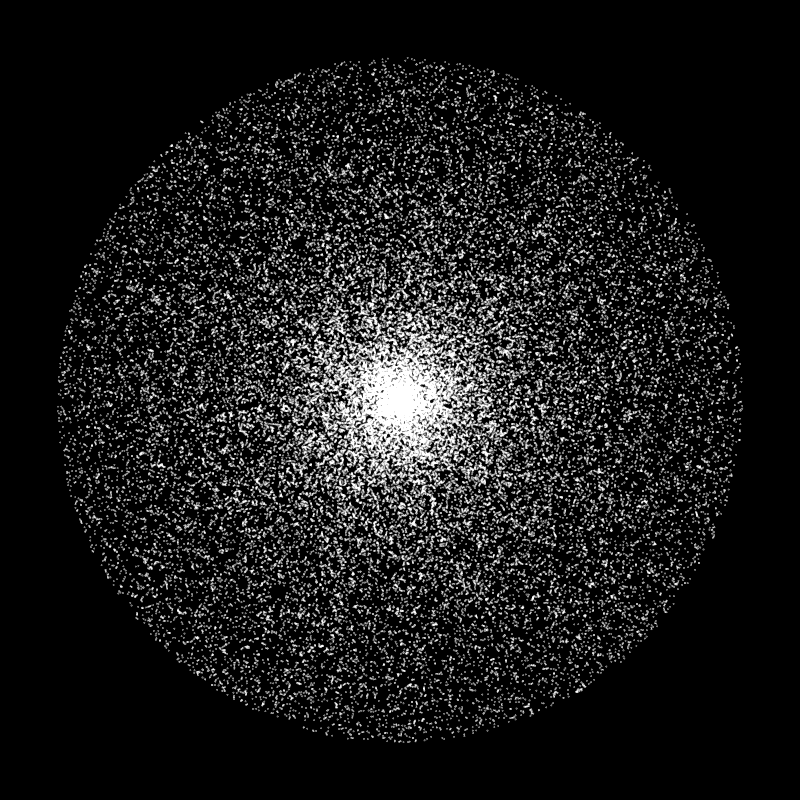
\includegraphics[width = 0.3 \textwidth]{img/galaxy-000.png}
  }
  \subfloat[1000]{
    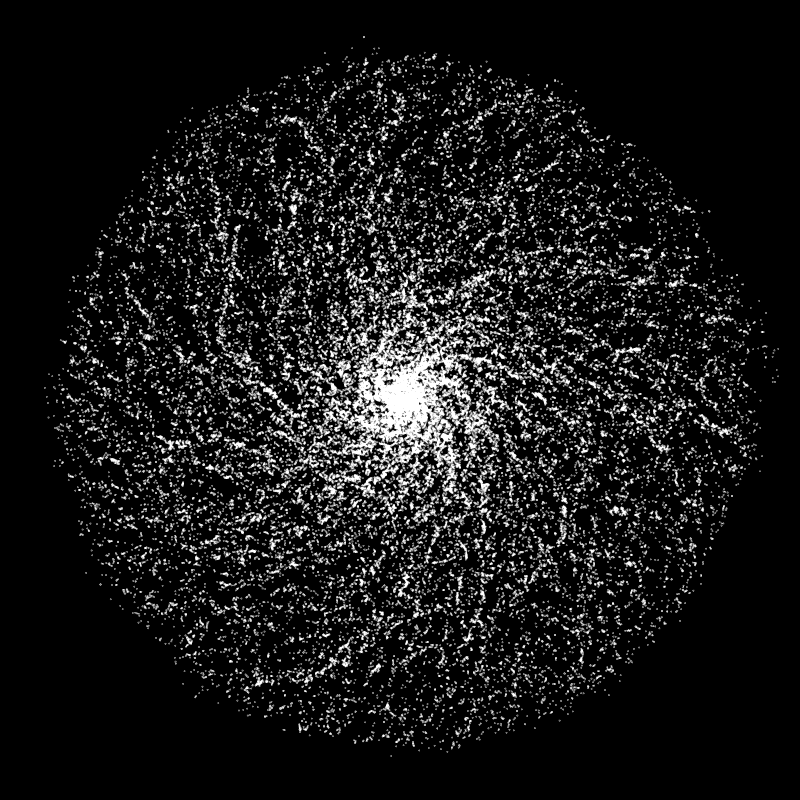
\includegraphics[width = 0.3 \textwidth]{img/galaxy-100.png}
  }
  \subfloat[2000]{
    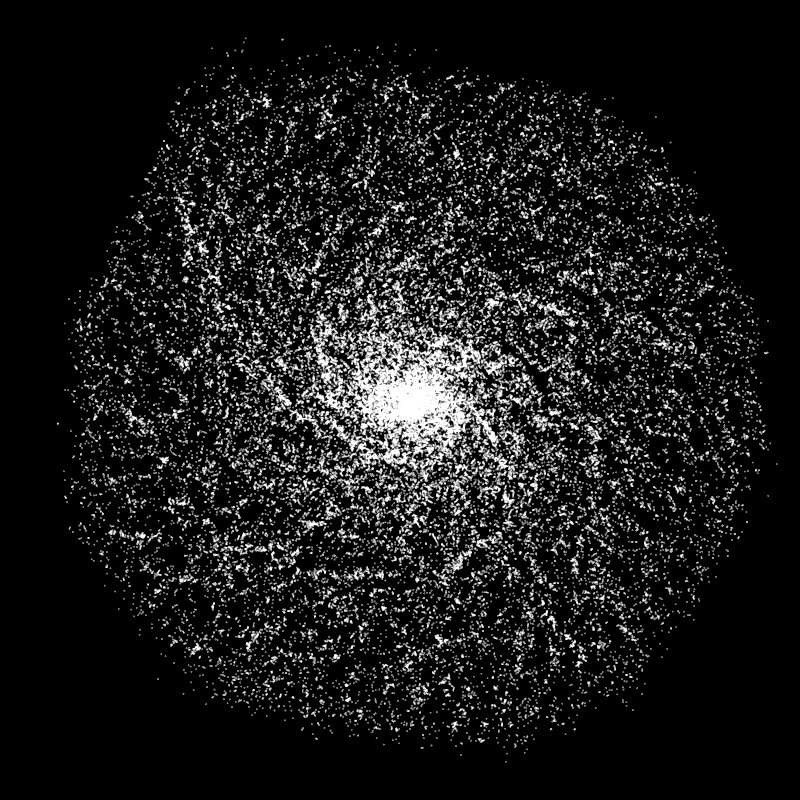
\includegraphics[width = 0.3 \textwidth]{img/galaxy-200.png}
  }

  \subfloat[3000]{
    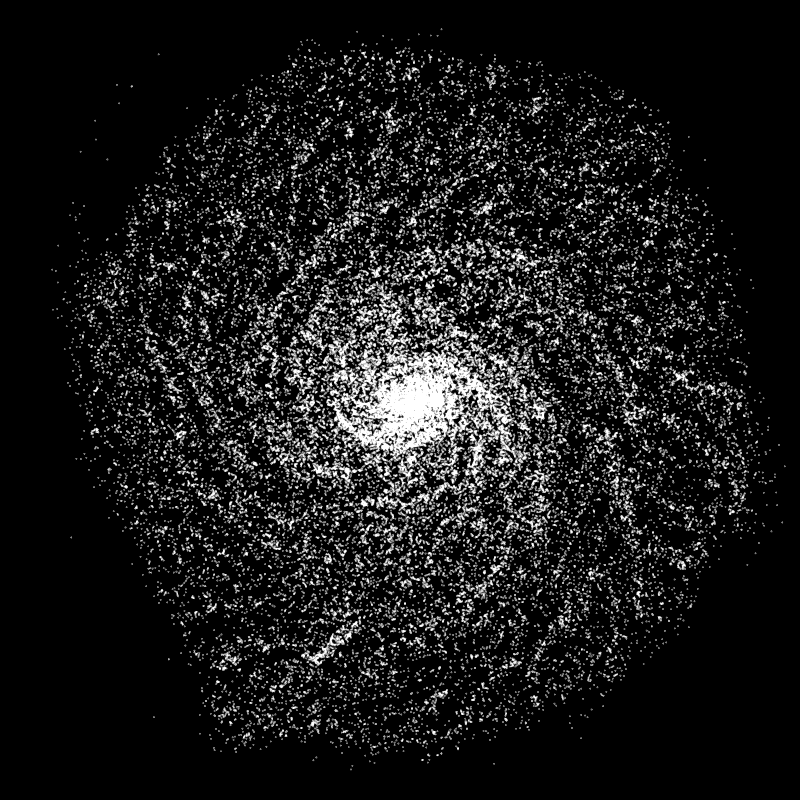
\includegraphics[width = 0.3 \textwidth]{img/galaxy-300.png}
  }
  \subfloat[4000]{
    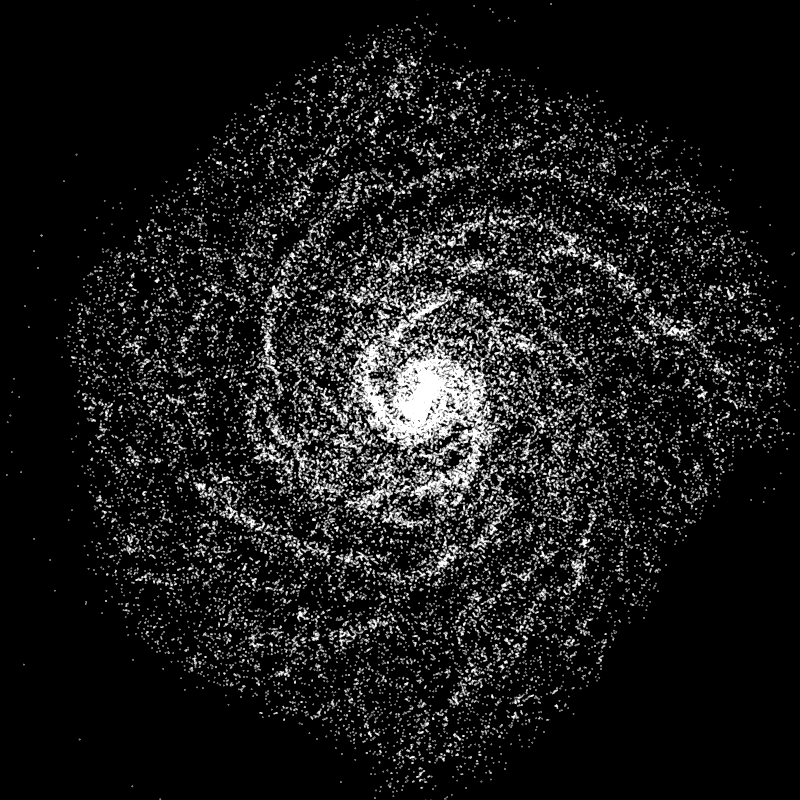
\includegraphics[width = 0.3 \textwidth]{img/galaxy-400.png}
  }
  \subfloat[5000]{
    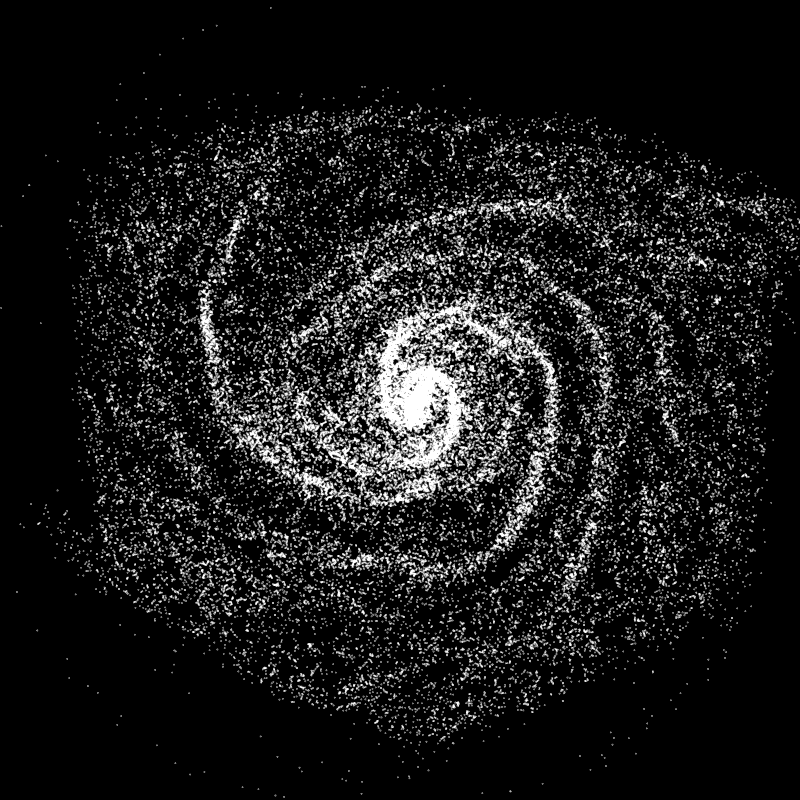
\includegraphics[width = 0.3 \textwidth]{img/galaxy-500.png}
  }
  \caption{Results of the galaxy simulation at different time steps.}
  \label{fig:res-galaxy}
\end{figure}

\begin{figure}
  \centering
  \subfloat[Scaling behavior with maximal 50 particles per leaf]{
    \label{fig:measure:n}
    \begin{tikzpicture}[scale=0.65]
      \begin{axis}[ xlabel = {Number of particles}
                  , ylabel = {Wall time [\si{s}]}
                  , xmode  = log
                  , ymode  = log
                  , width  = 0.7\textwidth
                  , height = 0.7\textwidth
                  , grid   = both
                  , grid style                    = {line width=.2pt, draw=gray!10}
                  , major grid style              = {line width=.2pt, draw=gray!50}
                  , legend pos                    = {north west}
                  , legend cell align             = {left}
                  , every axis plot/.append style = {ultra thick}
                  , cycle list name               = mark list
                  ]
        \addplot+[highlight] table [x=nParticles,y=time] {data/scaling_time-per-particles-leaf050-dt0.1-nSteps500.txt};
        \addlegendentry{Measurements};

        \addplot[ifi, domain=3e1:5e2] {x^2 * 2.45234e-6};
        \addplot[ifi, domain=5e2:1e6] {x   * 0.00122617};
        \fill[ifi] (500, 0.613085) circle (2pt);
        \addlegendentry{$\mathcal{O}(N^2)$ and $\mathcal{O}(N)$ for comparison};
      \end{axis}
    \end{tikzpicture}
  } \subfloat[Runtime for varying number of particles per leaf with $N = 2^{12}$]{
    \label{fig:measure:s}
    \begin{tikzpicture}[scale=0.65]
      \begin{axis}[ xlabel = {Maximum number of particles per leaf}
                  , ylabel = {Wall time [\si{s}]}
                  , width  = 0.7\textwidth
                  , height = 0.7\textwidth
                  , grid   = both
                  , grid style                    = {line width=.2pt, draw=gray!10}
                  , major grid style              = {line width=.2pt, draw=gray!50}
                  , minor x tick num              = 1
                  , minor y tick num              = 1
                  , every axis plot/.append style = {ultra thick}
                  , cycle list name               = mark list
                  ]
        \addplot+[highlight] table [x=s,y=time] {data/time-per-s-n04e3-dt0.1-nSteps500.txt};
      \end{axis}
    \end{tikzpicture}
  }
  \caption{Measured runtime with varying number of particles and maximum particles per leaf node}
\end{figure}

In \cref{fig:measure:n} you can see the scaling behavior of the \gls{fmm} for our galaxy example with maximal 50 particles per leaf node.
For easier interpretation we also show how quadratic and linear scaling would look like.
For small number of particles ($N < 500$) the algorithm scales approximately quadratically.
This is to be expected since all particles could fit into ten leaves which means that almost all interactions are calculated directly.
On the other hand, we see that the complexity approaches $\mathcal{O}(N)$ for larger $N$.

Furthermore, we investigate the effect that the maximum number $s$ of particles per leaf has on the runtime.
\cref{fig:measure:s} collects benchmark results for $N = 2^{12} = 4096$.
We observe the shortest runtimes with values of $s$ between 25 and 64.
The optimum among the tested values is $s=50$, which reduces the runtime by a factor of six compared to $s=1$.


  \clearpage
  \bibliographystyle{abbrv}
  \bibliography{references}
  \nocite{*}
\end{document}
